 \documentclass[t]{beamer}
%\documentclass[c]{beamer}
\listfiles

\mode<presentation>
{
  \usetheme[english,titlepage0]{KIT}
% \usetheme[usefoot]{KIT}
% \usetheme{KIT}

%%  \usefonttheme{structurebold}

  \setbeamercovered{transparent}

  %\setbeamertemplate{enumerate items}[circle]
  \setbeamertemplate{enumerate items}[ball]

}
\usepackage{babel}
%\date{10.05.2010}
%\DateText

\newlength{\Ku}
\setlength{\Ku}{1.43375pt}

\usepackage[latin1]{inputenc}
\usepackage[TS1,T1]{fontenc}
\usepackage{array}
\usepackage{multicol}
\usepackage{lipsum}

%\usenavigationsymbols
%\usenavigationsymbols[sfHhdb]
%\usenavigationsymbols[sfhHb]

\title[]{Together to the Top}
%\subtitle{Karlsruhe Institute of Technology (KIT)}

\author[]{KIT}

\AuthorTitleSep{\relax}

\institute[]{KARLSRUHE INSTITUTE OF TECHNOLOGY (KIT)}
%\institute[\raisebox{-4mm}{\includegraphics[height=5mm]{images/OU-Logo}}]
%  {KARLSRUHE INSTITUTE OF TECHNOLOGY (KIT)}
%\logo{\includegraphics[height=12mm]{images/OU-Logo}}

\TitleImage[width=\titleimagewd]{images/KIT-Titel}

\newlength{\tmplen}

\newcommand{\verysmall}{\fontsize{6pt}{8.6pt}\selectfont}

\begin{document}

\begin{frame}
  \maketitle
\end{frame}

\begin{frame}
  \frametitle{Unique Cooperation}

  Karlsruhe Institute of Technology (KIT):
  \settowidth{\tmplen}{Forschungszentrum Karlsruhe GmbH}
  \addtolength{\tmplen}{-\textwidth}
  \setlength{\tmplen}{-\tmplen}
  \vspace{50mm}

  The cooperation of\\
  Forschungszentrum Karlsruhe GmbH\\
  and Universit�t Karlsruhe (TH)\\
  \hfill
  \parbox{\tmplen}{\vbox to 0pt{\vss
\includegraphics[width=\tmplen]
        {images/KIT-Kooperation}}}
\end{frame}

\begin{frame}
  \frametitle{Two Strong Partners}

  \small
  \renewcommand{\baselinestretch}{.95}\selectfont
  \begin{minipage}{.625\linewidth}
    \heading{Forschungszentrum Karlsruhe:}
    \begin{itemize}
    \item Programmatic research on highest international level
    \item One of the largest and most successful science and engineering
          research institutions in Europe
    \item Member of the Helmholtz Association of National Research Centers
    \end{itemize}

    \heading{Universit�t Karlsruhe (TH):}
    \begin{itemize}
    \item Winner of the Excellence Initiative 2006 launched by the Federal
          Republic of Germany and the federal states
    \item One of the universities strongest in research worldwide
    \item Highest acquisition of DFG third-party funds per capita in Germany
    \end{itemize}
  \end{minipage}
  \hfill
  \parbox{.325\linewidth}{\makebox[.325\textwidth][r]{
      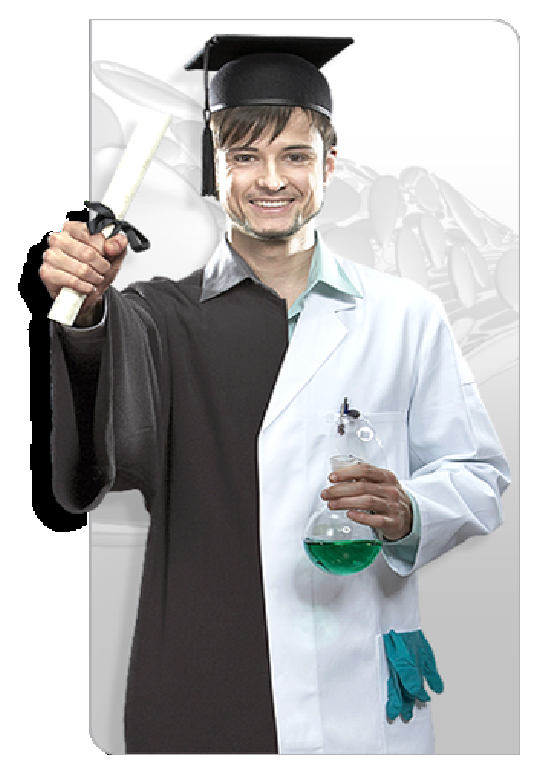
\includegraphics[width=.375\textwidth]
        {images/KIT-Promotion}}}
\end{frame}

\begin{frame}
  \frametitle{Common Objective}

  Positioning as an institution of excellent research and lecturing in
  natural and engineering sciences on an international scale,
  with worldwide top scientific excellence in
  \bigskip
  %\bigskip
  
  \parbox{.2875\linewidth}{%
    
\includegraphics[width=.2875\textwidth]
      {images/KIT-Research}
    \begin{itemize}\item Research\end{itemize}}
  \hfill
  \parbox{.2875\linewidth}{%
    
\includegraphics[width=.2875\textwidth]
      {images/KIT-Teaching}
    \begin{itemize}\item Teaching\end{itemize}}
  \hfill
  \parbox{.2875\linewidth}{%
    
\includegraphics[width=.2875\textwidth]
      {images/KIT-Innovation}
    \begin{itemize}\item Innovation\end{itemize}}
\end{frame}

\begin{frame}
  \frametitle{Competence Portfolio}

  \parbox{.64\textwidth}{\raggedright
    Excellent research is based above all on the skills and knowledgeof
    the scientific employees.
    \bigskip

    In KIT these scientists will work in fields of competence depending
    on their expert know-how. Related fields of competence are bundled
    in competence areas.
    \bigskip

    Fields of competence and competence areas make up the competence
    portfolioof KIT. It is dynamic and will develop and take up new
    scientific topics.}
  \hfill
  \parbox{.312\textwidth}{%
    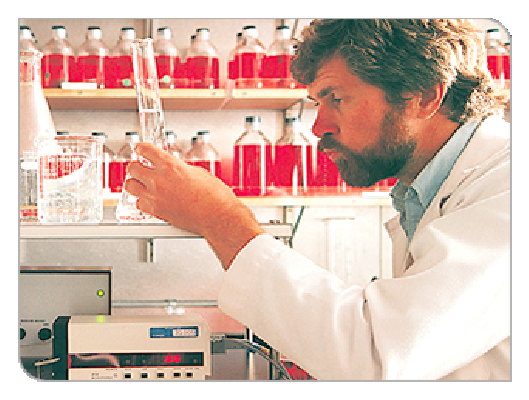
\includegraphics[width=.312\textwidth]
      {images/KIT-Labor1}\\
    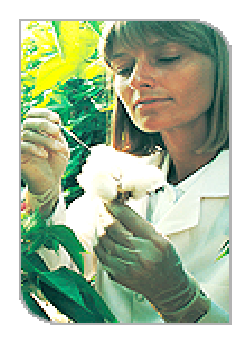
\includegraphics[width=.133\textwidth]
      {images/KIT-Labor2}
    \hfill
    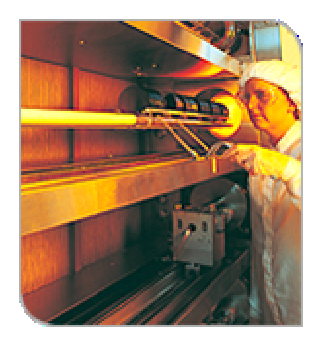
\includegraphics[width=.176\textwidth]
      {images/KIT-Labor3}}
\end{frame}

\begin{frame}
  \frametitle{Competence Portfolio}
  \framesubtitle{\normalsize\mdseries 30 Fields of Competence Bundled
    in 6 Areas of Competence}

  \renewcommand{\baselinestretch}{.8}\scriptsize%\selectfont
  \begin{tikzpicture}
    % Matter and Materials
    \draw[KITblack50,fill=KITblack30,line width=.5\Ku]
      (0\Ku,135\Ku) rectangle
      (74\Ku,126\Ku)
      (37\Ku,130.5\Ku) node {\color{black}Matter and Materials};
    \draw[KITblack50,fill=KITblack15,line width=.5\Ku]
      (0\Ku,126\Ku) rectangle
      (74\Ku,87\Ku);
    \pgftext[at=\pgfpoint{2\Ku}{124.6\Ku},top,left]{%
      \parbox{72\Ku}{%
	\begin{itemize}\verysmall\itemsep=0pt\parsep=0pt
        \item Elementary Particle and Astroparticle Physics
        \item Condensed Matter
        \item Nanoscience
        \item Microtechnology
        \item Optics and Photonics
        \item Applied and New Materials
        \end{itemize}}}
    % Earth and Environment
    \draw[KITblack50,fill=KITblack30,line width=.5\Ku]
      (77\Ku,135\Ku) rectangle
      (151\Ku,126\Ku)
      (114\Ku,130.5\Ku) node {\color{black}Earth and Environment};
    \draw[KITblack50,fill=KITblack15,line width=.5\Ku]
      (77\Ku,126\Ku) rectangle
      (151\Ku,87\Ku);
    \pgftext[at=\pgfpoint{79\Ku}{128.5\Ku},top,left]{%
      \parbox{70\Ku}{%
	\begin{itemize}\verysmall\itemsep=0pt\parsep=0pt
        \item Atmosphere and Climate
        \item Geosphere and Risk Management
        \item Hydrosphere and Environmental Engineering
        \item Constructed Facilities and Urban Infrastructure
        \end{itemize}}}
    % Applied Life Sciences
    \draw[KITblack50,fill=KITblack30,line width=.5\Ku]
      (154\Ku,135\Ku) rectangle
      (230\Ku,126\Ku)
      (192\Ku,130.5\Ku) node {\color{black}Applied Life Sciences};
    \draw[KITblack50,fill=KITblack15,line width=.5\Ku]
      (154\Ku,126\Ku) rectangle
      (230\Ku,87\Ku);
    \pgftext[at=\pgfpoint{156\Ku}{128.5\Ku},top,left]{%
      \parbox{74\Ku}{%
	\begin{itemize}\verysmall\itemsep=0pt\parsep=0pt
        \item Biotechnology
        \item Toxicology and Food Science
        \item Health and Medical Engineering
        \item Cellular and Structural Biology
        \end{itemize}}}
    % Systems and Processes
    \draw[KITblack50,fill=KITblack30,line width=.5\Ku]
      (0\Ku,84\Ku) rectangle
      (230\Ku,75\Ku)
      (115\Ku,79.5\Ku) node {\color{black}Systems and Processes};
    % links:
    \draw[KITblack50,fill=KITblack15,line width=.5\Ku]
      (0\Ku,75\Ku) rectangle
      (115\Ku,51\Ku);
    \pgftext[at=\pgfpoint{2\Ku}{77.5\Ku},top,left]{%
      \parbox{111\Ku}{%
	\begin{itemize}\verysmall\itemsep=0pt\parsep=0pt
        \item Fluid and Particle Dynamics
        \item Chemical and Thermal Process Engineering
        \item Fuels and Combustion
        \end{itemize}}}
    % rechts:
    \draw[KITblack50,fill=KITblack15,line width=.5\Ku]
      (115\Ku,75\Ku) rectangle
      (230\Ku,51\Ku);
    \pgftext[at=\pgfpoint{117\Ku}{77.5\Ku},top,left]{%
      \parbox{111\Ku}{%
	\begin{itemize}\verysmall\itemsep=0pt\parsep=0pt
        \item Systems and Embedded Systems
        \item Power Plant Technology
        \item Product Life Cycle
        \item Mobile Systems and Mobility Engineering
        \end{itemize}}}
    % Information, Communication, and Organization
    \draw[KITblack50,fill=KITblack30,line width=.5\Ku]
      (0\Ku,48\Ku) rectangle
      (111\Ku,39\Ku)
      (55.5\Ku,43.5\Ku) node {\color{black}Information, Communication, and Organization};
    \draw[KITblack50,fill=KITblack15,line width=.5\Ku]
      (0\Ku,39\Ku) rectangle
      (111\Ku,4\Ku);
    \pgftext[at=\pgfpoint{2\Ku}{41.5\Ku},top,left]{%
      \parbox{109\Ku}{%
	\begin{itemize}\verysmall\itemsep=0pt\parsep=0pt
        \item Algorithm, Software, and System Engineering
        \item Cognition and Information Engineering
        \item Communication Technology
        \item High-Performance and Grid Computing
        \item Mathematical Models
        \item Organization and Service Engineering
        \end{itemize}}}
    % Technology, Culture, and Society
    \draw[KITblack50,fill=KITblack30,line width=.5\Ku]
      (119\Ku,48\Ku) rectangle
      (230\Ku,39\Ku)
      (174.5\Ku,43.5\Ku) node {\color{black}Technology, Culture, and Society};
    \draw[KITblack50,fill=KITblack15,line width=.5\Ku]
      (119\Ku,39\Ku) rectangle
      (230\Ku,4\Ku);
    \pgftext[at=\pgfpoint{119\Ku}{41.5\Ku},top,left]{%
      \parbox{109\Ku}{%
	\begin{itemize}\verysmall\itemsep=0pt\parsep=0pt
	\item Cultural Heritage and Dynamics of Change
	\item Business Organization and Innovation
	\item Interaction of Science and Technology with Society
	\end{itemize}}}
  \end{tikzpicture}
  \renewcommand{\baselinestretch}{1}\selectfont
\end{frame}

\begin{frame}
  \frametitle{Innovative Research Structures}

  \parbox{.65\textwidth}{%
    KIT-Centers:
    \begin{itemize}
      \item Energy
      \item Nano \& Micro Science and Technology
      \item Elementary Particle and Astroparticle Physics
      \item Climate and Environment
    \end{itemize}
    \bigskip

    KIT-Focuses:
    \begin{itemize}
      \item COMMputation
      \item Mobility Systems
      \item Optics and Photonics
      \item Humans and Technology
      \item Applied and New Materials
    \end{itemize}}
  \hfill
  \parbox{.3\textwidth}{%
    
\includegraphics[width=.3\textwidth]
      {images/KIT-Zentren}\\
    \parbox{.135\textwidth}{%
    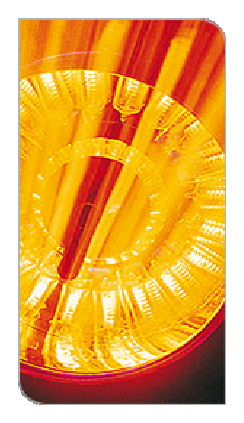
\includegraphics[width=.14\textwidth]
      {images/KIT-Schwerpunkt1}}%
    \hfill
    \parbox{.149\textwidth}{%
      \hspace*{-.005\textwidth}%
      
\includegraphics[width=.154\textwidth]
        {images/KIT-Schwerpunkt2}\\
      \hspace*{-.005\textwidth}%
      
\includegraphics[width=.154\textwidth]
        {images/KIT-Schwerpunkt3}
      \vspace*{.055\textwidth}}}
\end{frame}

\begin{frame}
  \frametitle{Figures}

  \vspace*{10\Ku}
  \begin{tabular}[b]{r}
    Employees\phantom{m} \\
    \resizebox{68\Ku}{!}{\bfseries\color{KITgreen}8.000}
  \end{tabular}
  \hspace{15\Ku}
  \begin{tabular}[b]{r@{\hspace{-.2em}}l}
    & Students \\
    \resizebox{100\Ku}{!}{\bfseries\color{KITblack50}19.895}
  \end{tabular}\\[-1\Ku]
  \hfill
  \raisebox{7\Ku}{%
    \begin{tabular}{r}
      \resizebox{52\Ku}{!}{\bfseries 350\phantom{0}} \\
      Professors
    \end{tabular}}
  \hspace{1\Ku}
  \begin{tabular}{l}
    \resizebox{72\Ku}{!}{\bfseries\color{KITgreen}650} \\
    \hspace*{12.5\Ku}annual budget in Million Euros
  \end{tabular}
  \bigskip

  
\includegraphics[height=35\Ku]{images/KIT-Liste1}
  \hspace{1\Ku}
  
\includegraphics[height=35\Ku]{images/KIT-Liste2}
\end{frame}

\begin{frame}
  \frametitle{Karlsruher Institute of Technology}

  \vspace*{10\Ku}
  Thank you for your attention.
  \bigskip

  
\includegraphics[width=\textwidth]{images/KIT-Finale-c}
\end{frame}
\end{document}
